\chapter{Data Warehouse Design and Implementation}
\section{Source Database Design}
In the raw operational form, answering a question such as ``what is the default rate for a given district and loan-size band?'' requires joining several normalised tables and re-deriving every measure each time. The source CSVs were parsed, mapped to common keys, and cleaned before being loaded into the target warehouse schema. The dimensional model separates measurements (facts) from context (dimensions), so the same measures can be reused across different analyses.

\section{Dimensional Modeling (Galaxy Schema)}
To accommodate both transaction metrics and loan metrics, a \textbf{Galaxy Schema} was implemented: an advanced evolution of the star schema in which multiple fact tables share conformed dimensions. Each fact table with its dimensions forms a star; together the two stars form a galaxy, allowing loan and transaction behaviour to be compared on the same date, account, and branch.

\subsection{Dimension Tables (Context)}
\begin{itemize}
    \item \texttt{dim\_date}: Conformed date dimension covering 2,191 days (year, quarter, month, day, weekday, weekend flag).
    \item \texttt{dim\_branch}: 77 district/branch rows with city, region, and urban/rural type.
    \item \texttt{dim\_customer}: 5,369 clients with age, age group, gender, and home branch.
    \item \texttt{dim\_account}: 4,500 accounts with owner, account type, and open date.
    \item \texttt{dim\_loan\_type}: A single explicit \texttt{Unspecified} member, because the source contains no loan product category or interest rate.
\end{itemize}

\subsection{Fact Tables (Measurements)}
\begin{itemize}
    \item \texttt{fact\_transactions}: 1,056,320 rows, one per account transaction. Grain is the individual transaction; measures are amount and resulting balance.
    \item \texttt{fact\_loans}: 682 rows, one per loan. Measures are principal amount, duration, payments, and status. The interest-rate column is present but null for every row.
\end{itemize}

\begin{table}[H]
    \centering
    \renewcommand{\arraystretch}{1.3}
    \begin{tabularx}{\textwidth}{|>{\raggedright\arraybackslash}l|>{\raggedright\arraybackslash}l|>{\raggedright\arraybackslash}X|}
        \hline
        \textbf{Column Name} & \textbf{Data Type} & \textbf{Description} \\
        \hline
        \texttt{transaction\_id} & \texttt{BIGINT} (PK) & Unique identifier for the transaction. \\
        \texttt{account\_id} & \texttt{INT} (FK) & Reference to \texttt{dim\_account}. \\
        \texttt{date\_id} & \texttt{INT} (FK) & Reference to \texttt{dim\_date} for the transaction date. \\
        \texttt{branch\_id} & \texttt{INT} (FK) & Reference to \texttt{dim\_branch} for the account's district. \\
        \texttt{transaction\_type} & \texttt{VARCHAR} & Deposit or Withdrawal. \\
        \texttt{amount} & \texttt{NUMERIC} & Transaction amount. \\
        \texttt{balance} & \texttt{NUMERIC} & Account balance after the transaction. \\
        \hline
    \end{tabularx}
    \caption{Data dictionary: \texttt{fact\_transactions}}
    \label{tab:dict_transactions}
\end{table}

\begin{table}[H]
    \centering
    \renewcommand{\arraystretch}{1.3}
    \begin{tabularx}{\textwidth}{|>{\raggedright\arraybackslash}l|>{\raggedright\arraybackslash}l|>{\raggedright\arraybackslash}X|}
        \hline
        \textbf{Column Name} & \textbf{Data Type} & \textbf{Description} \\
        \hline
        \texttt{loan\_id} & \texttt{INT} (PK) & Unique identifier for the loan record. \\
        \texttt{account\_id} & \texttt{INT} (FK) & Reference to \texttt{dim\_account}. \\
        \texttt{customer\_id} & \texttt{INT} (FK) & Reference to \texttt{dim\_customer} for the account owner. \\
        \texttt{branch\_id} & \texttt{INT} (FK) & Reference to \texttt{dim\_branch}. \\
        \texttt{loan\_type\_id} & \texttt{INT} (FK) & Reference to \texttt{dim\_loan\_type} (always the Unspecified member). \\
        \texttt{date\_id} & \texttt{INT} (FK) & Reference to \texttt{dim\_date} for the loan date. \\
        \texttt{amount} & \texttt{NUMERIC} & Principal disbursed. \\
        \texttt{tenure\_months} & \texttt{INT} & Agreed loan duration. \\
        \texttt{payments} & \texttt{INT} & Number of instalments. \\
        \texttt{status} & \texttt{VARCHAR} & Closed, Active, or Defaulted. \\
        \hline
    \end{tabularx}
    \caption{Data dictionary: \texttt{fact\_loans}}
    \label{tab:dict_loans}
\end{table}

\begin{figure}[H]
    \centering
    \resizebox{\textwidth}{!}{
    \begin{tikzpicture}[
        >=Stealth,
        every node/.style={font=\sffamily\small},
        tablePrimary/.style={
            rectangle split, rectangle split parts=2,
            draw=midgray!50, thick,
            rectangle split part fill={primary, white},
            rounded corners=4pt, text width=4.2cm, align=left,
            inner sep=1.5ex
        },
        tableSecondary/.style={
            rectangle split, rectangle split parts=2,
            draw=midgray!50, thick,
            rectangle split part fill={secondary, white},
            rounded corners=4pt, text width=4.2cm, align=left,
            inner sep=1.5ex
        },
        line/.style={draw, thick, color=midgray, -{Latex[length=2mm, width=2mm]}}
    ]

    % Fact Loans
    \node[tablePrimary] (floans) at (-4, 6) {
        \hfil \textbf{\textcolor{white}{fact\_loans}} \hfil
        \nodepart{two}
        \texttt{int} \textbf{loan\_id} [PK]\\
        \texttt{numeric} amount\\
        \texttt{int} tenure\_months\\
        \texttt{varchar} status
    };

    % Fact Transactions
    \node[tablePrimary] (ftrans) at (6, 6) {
        \hfil \textbf{\textcolor{white}{fact\_transactions}} \hfil
        \nodepart{two}
        \texttt{bigint} \textbf{transaction\_id} [PK]\\
        \texttt{numeric} amount\\
        \texttt{varchar} transaction\_type
    };

    % Dim Loan Type
    \node[tableSecondary] (dltype) at (-9, 0) {
        \hfil \textbf{\textcolor{white}{dim\_loan\_type}} \hfil
        \nodepart{two}
        \texttt{int} \textbf{loan\_type\_id} [PK]\\
        \texttt{varchar} loan\_type\_name
    };

    % Dim Customer
    \node[tableSecondary] (dcust) at (-4, 0) {
        \hfil \textbf{\textcolor{white}{dim\_customer}} \hfil
        \nodepart{two}
        \texttt{int} \textbf{customer\_id} [PK]\\
        \texttt{varchar} gender\\
        \texttt{varchar} age\_group\\
        \texttt{int} home\_branch\_id
    };

    % Dim Date
    \node[tableSecondary] (ddate) at (1, 0) {
        \hfil \textbf{\textcolor{white}{dim\_date}} \hfil
        \nodepart{two}
        \texttt{int} \textbf{date\_id} [PK]\\
        \texttt{date} full\_date\\
        \texttt{int} year\\
        \texttt{int} quarter\\
        \texttt{varchar} month\_name
    };

    % Dim Branch
    \node[tableSecondary] (dbranch) at (6, 0) {
        \hfil \textbf{\textcolor{white}{dim\_branch}} \hfil
        \nodepart{two}
        \texttt{int} \textbf{branch\_id} [PK]\\
        \texttt{varchar} branch\_name\\
        \texttt{varchar} city\\
        \texttt{varchar} region
    };

    % Dim Account
    \node[tableSecondary] (dacc) at (11, 0) {
        \hfil \textbf{\textcolor{white}{dim\_account}} \hfil
        \nodepart{two}
        \texttt{int} \textbf{account\_id} [PK]\\
        \texttt{int} customer\_id\\
        \texttt{varchar} account\_type
    };

    % Relations (Fact Loans)
    \draw[line] (floans.south) -- (dltype.north);
    \draw[line] (floans.south) -- (dcust.north);
    \draw[line] (floans.south) -- (ddate.north);
    \draw[line] (floans.south) -- (dbranch.north);

    % Relations (Fact Transactions)
    \draw[line] (ftrans.south) -- (ddate.north);
    \draw[line] (ftrans.south) -- (dbranch.north);
    \draw[line] (ftrans.south) -- (dacc.north);

    \end{tikzpicture}
    }
    \caption{Galaxy schema for the banking data warehouse}
    \label{fig:galaxy_schema}
\end{figure}

\section{Warehouse Implementation}
The ETL pipeline builds dimensions first and facts second, so every fact row resolves to a surrogate dimension key. The generated warehouse diagram is shown in Figure~\ref{fig:galaxy_png}; the dashboard data-model card, which lists join keys and a column dictionary for the warehouse tables, is shown in Chapter~10 as Figure~\ref{fig:dashboard_datacard}.

\begin{figure}[H]
    \centering
    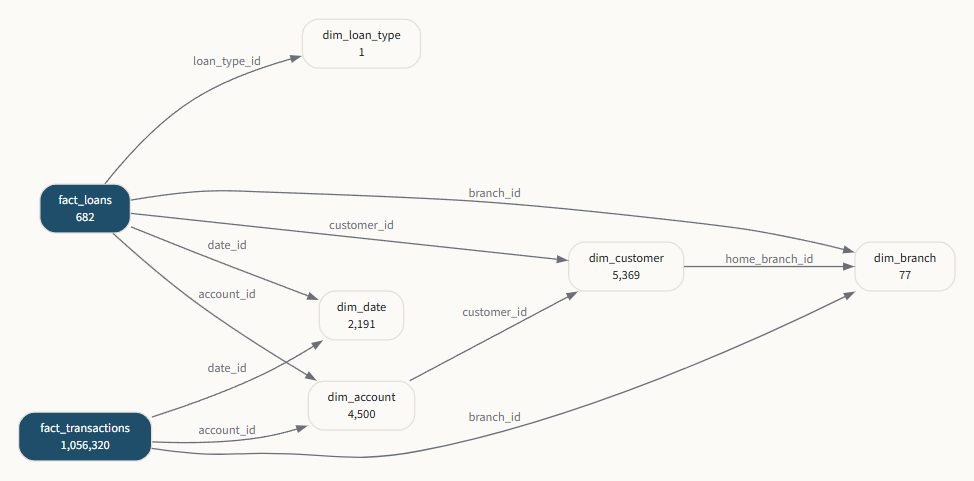
\includegraphics[width=0.9\textwidth]{figures/18_galaxy_schema.png}
    \caption{Generated galaxy-schema diagram used in the dashboard}
    \label{fig:galaxy_png}
\end{figure}

\section{Analytical Queries}
Reporting queries are executed against the modelled tables through the Snowflake reporting views introduced in Chapter~4, and the dashboard performs its own grouped aggregations for its charts. Representative analyses include default rate by branch, monthly transaction totals by type, and balance-based risk quadrants. These queries use ordinary grouping against the conformed dimensions; the focus of this project is the decision-support pipeline rather than a precomputed OLAP cube.
